\documentclass[12pt]{scrartcl}
\usepackage[utf8]{inputenc}
\usepackage[english,croatian]{babel} % neki citati su na izvornom engleskom, ali hrvatski je naravno glavni jezik eseja
\usepackage[unicode]{hyperref}
\usepackage{amsmath,amssymb,amsthm}
\usepackage{mathtools}
\usepackage{thmtools}
\usepackage{csquotes}
\usepackage{xcolor}
\usepackage[backend=biber]{biblatex}
\usepackage{algorithm}
\usepackage{algpseudocode}
\usepackage{listings}

\definecolor{codegreen}{rgb}{0,0.6,0}
\definecolor{codegray}{rgb}{0.5,0.5,0.5}
\definecolor{codepurple}{rgb}{0.58,0,0.82}
\definecolor{backcolour}{rgb}{0.95,0.95,0.92}

\lstdefinestyle{mystyle}{
    backgroundcolor=\color{backcolour},   
    commentstyle=\color{codegreen},
    keywordstyle=\color{magenta},
    numberstyle=\tiny\color{codegray},
    stringstyle=\color{codepurple},
    basicstyle=\ttfamily\footnotesize,
    breakatwhitespace=false,         
    breaklines=true,                 
    captionpos=b,                    
    keepspaces=true,                 
    numbers=left,                    
    numbersep=5pt,                  
    showspaces=false,                
    showstringspaces=false,
    showtabs=false,                  
    tabsize=2
}

\lstset{style=mystyle}
\renewcommand\lstlistingname{Implementacija}
\renewcommand\lstlistlistingname{Implementacije}
\def\lstlistingautorefname{Impl.}

\hypersetup{
    colorlinks,
    linkcolor={red!50!black},
    citecolor={blue!50!black},
    urlcolor={blue!80!black}
}

\addbibresource{literatura.bib}
\MakeOuterQuote{"}
\declaretheorem{teorem}
\declaretheorem[sibling=teorem]{lema}
\declaretheorem[style=definition,sibling=teorem,qed=$\vartriangleleft$]{definicija}
\declaretheorem[name=Primjer,style=definition]{example}

\newcommand{\T}{^\mathsf T}
\newcommand{\mat}[1]{%
    \ifmmode%
        \mathbf{#1}%
    \else%
        $\mathbf{#1}$%
    \fi%
}
\newcommand{\vek}[1]{\mat{#1}}
\newcommand{\citat}[2]{\begin{quotation}\textit{#1}\end{quotation}\begin{flushright}---#2\end{flushright}}
\newcommand{\primjer}[2]{%
    \renewcommand\qedsymbol{$\vartriangleleft$}%
    \begin{example}%
        #1%
    \end{example}%
    \begin{proof}[Rješenje]%
        #2%
    \end{proof}%
    \renewcommand\qedsymbol{$\square$}
}

\newcommand{\algoritam}[2]{%
\begin{algorithm}
\floatname{algorithm}{Algoritam}
\caption{#1}
\begin{algorithmic}
#2
\end{algorithmic}
\end{algorithn}
}

\title{Korijen --- 1 algoritam, 3 implementacije}
\date{\today}

\begin{document}
\maketitle
\tableofcontents
\pagebreak

\section{Uvod}
%V1:Ovaj esej se bavi naoko jednostavnim i elementarnim numeričkim algoritmom: računom kvadratnog korijena. Iako u osnovi poznat tisućama godina,
%ovaj algoritam ima fascinantan broj varijacija, što u njegovoj osnovnoj konceptualizaciji neovisnoj o namijenjenom izvršitelju, što u konkretnim
%formama koje dobiva u ovisnosti o različitim računalnim arhitekturama na kojima se povijesno implementirao.
Izračunati kvadratni korijen realnog broja --- koliko bi to moglo biti teško? Iako u osnovi poznat tisućama godina,
ovaj algoritam ima fascinantan broj varijacija, što u njegovoj osnovnoj konceptualizaciji neovisnoj o namijenjenom izvršitelju, što u konkretnim
formama koje dobiva u ovisnosti o različitim računalnim arhitekturama na kojima se povijesno implementirao.

U ovom eseju obrađujemo u detalje ovaj algoritam kroz povijest, od nekoliko stoljeća prije Krista
do današnjeg kompjutoriziranog doba u kojem su precizne i vrlo efikasne varijante
ovog algoritma od presudne važnosti u raznolikim poljima primjene, poput simulacije, digitalne fizike i računalne grafike. Usput ćemo predstaviti
i neke analize posebno zanimljivih modernih računalnih implementacija te predstaviti mjerenja obavljena na današnjim računalima za različite implementacije.

Pogledat ćemo dvije bitno različite klase algoritama za račun korijena: one namijenjene dobivanju \emph{cjelobrojnog} korijena i općenite
metode koje daju realan broj (u nekoj reprezentaciji s pomičnim zarezom). Iako je moguće dobiti određenu vrstu povećane preciznosti
cjelobrojnih algoritama korištenjem brojeva s fiksnim zarezom, takvi algoritmi nisu primjenjivi na jako velikom rasponu brojeva jer uvijek moramo
fiksno odvojiti cijeli i ne-cijeli dio. Zato se na kraju se bavimo specifično algoritmom koji je namijenjen računu u realnim
brojevima i samim time mora koristiti reprezentaciju realnih brojeva pomoću \emph{pomičnog} zareza, dostupnu u većini današnjih računala.
Sljedeća definicija će biti od koristi kroz cijeli rad:
\begin{definicija}
    Neka je $N\in\mathbb{N}$. Kažemo da je $x$ cjelobrojni (kvadratni) korijen od $N$ ako vrijedi
    \begin{equation*}
        x^2 \leq N < (x+1)^2\text.
    \end{equation*}
\end{definicija}

\section{Povijest računa kvadratnog korijena}\label{sec:hist}
    \citat{\begin{otherlanguage}{english}
        Seeing there is nothing that is so troublesome to Mathematicall practise, nor that doth more molest and hinder Calculators,
    then the Multiplications, Diuisions, square and cubical Extractions of great numbers, which besided the tedious expence
    of time, are for the most part subiect to many slippery errors. I began therefore to consider in my minde, by what certaine
    and ready Art I might remoue those hindrances~\cite[str.~194]{taocp2}.
    \end{otherlanguage}}{John Napier (1616.)}

\subsection{Babilonski period}

Najstariji poznati zapisi netrivijalnih numeričkih algoritama "u akciji" potiču iz drevnog Babilona --- poznato
 je da su babilonski matematičari znali računati zbroj, razliku, umnožak, recipročnu vrijednost te kvadratni korijen brojeva prikazanih
u \emph{seksagezimalnom} (baza $60$) brojevnom sustavu; potonje dvije stavke su pak mogli računati svojevrsnom linearnom interpolacijom iz
sastavljenih tablica, ili preciznije, ploča. Naime, ekskavirane su razne ploče s korespondencijom između brojeva $n$ i $n^2$. Korektne ploče s
recipročnim vrijednostima brojeva su pronađene samo za "regularne" brojeve do određene duljine, tj.\ one s konačnim prikazom u seksagezimalnom sustavu, jer
se čini da Babilonjani nisu poznavali ponavljajuće nizove znamenki~\cite{KnuthBabylon}.

Valja napomenuti da je starobabilonski brojevni sustav
također podrazumijevao rad u jednoj vrsti "pomičnog zareza" koja se temelji na činjenici da bilo koji zapisan broj može odjednom predstaviti
\emph{bilo koji} svoj umnožak sa $60^k,\,k\in\mathbb{Z}$. Iako nam ovakav "nedeterminizam" danas može zvučati suviše složenim i svakako
neprikladnim za računalnu implementaciju, bio je ključan za relativno precizne rezultate do kakvih su starobabilonski matematičari redovito
dolazili, koristeći pritom donekle intuitivno očekivanje koliko bi brojevi trebali biti veliki ili mali u kontekstu u kojem se zadani račun rješava
(tipično je to bilo u sklopu nekog računa iz stvarnosti, sa zadanim jedinicama i očekivanim redom veličine dimenzija rezultata) kako bi mogli odrediti
prikladan faktor skaliranja u svakom međukoraku računa. Ovo znači da su svi aritmetički algoritmi iz tog doba radili podjednako dobro i za 
"realne" i za cijele brojeve, jer bi za praktičnu razliku između njih bila odgovorna osoba koja računa.

Zanimljivo je napomenuti da su pronađeni mnogi spisi koji potječu od oko 2.~stoljeća prije Krista u kojima
se rješavaju zadaci poput izračunavanja dimenzija cisterni sa zadanim ograničenjima, što je dovelo do impresivnih zapisa (koji podsjećaju
na današnje pseudokod-programe!) ručnog izvršavanja
 \emph{algoritama} za rješavanje linearnih, ali i složenijih sustava jednadžbi poput $x+y=a,\ x^2+y^2=b$, za što je očito bilo potrebno
imati ili algoritam za račun korijena ili odgovarajuću tablicu. Primjerice, Babilonjani su aproksimirali $\sqrt 2$ ($N=2$) na ovaj način (prevedeno
u dekadske razlomke)\cite{fowler1998}:
\begin{equation}\label{eq:babiter}
    \sqrt 2 = \sqrt{\left(\frac32\right)^2 - \frac14}\approx\frac32 - \frac12\times\frac14\times\frac23 = \frac32 - \frac{1}{12} = \frac{17}{12}\text.
\end{equation}
Račun započinje uzimanjem početne aproksimacije korijena, $a=\frac32$ u~\eqref{eq:babiter}, te uz pretpostavku da je ona veća od prave vrijednosti,
dodavanjem ostatka $B$ koji nam nije poznat, ali za kojeg znamo da mora biti manji od kvadrata početne aproksimacije. Modernim algebarskim riječnikom,
ovo odgovara
\[
    B=a^2-N,
\]
gdje odmah vidimo da ovo povlači $a-B+N<N$, što znači da smo sada dobili aproksimaciju koja je manja od prave vrijednosti. Pritom imamo dualnu situaciju
ako počnemo od manje aproksimacije; slika~\ref{sl:babiter} prikazuje najvjerojatniji način na koji su Babilonjani konstruirali i koristili ovaj postupak.
%TODO: slika ovdje, sa stranice 6 citiranog članka; prepiši u TikZ i prilagodi tekst!

Dakako, opisan bi račun, radi dobivanja veće preciznosti rezultata, trebalo iterirati,
uzimanjem dobivene ($\frac{17}{12}$ u~\eqref{eq:babiter}) bolje aproksimacije umjesto prethodne
($\frac32$) za nastavak računa, no zapisi s takvim postupcima nisu pronađeni,
vjerojatno zbog toga što se rijetko kada dobije "regularan" međurezultat te zbog toga što
bi potreban račun bio suviše složen, uključujući množenja za koja nisu postojali podaci u dostupnim tablicama za množenje. Stoga se čini da su 
Babilonjani bili uglavnom zadovoljni rezultatom jedne jedine iteracije ove osnovne metode, koja je u biti ekvivalentna mnogo kasnije zabilježenom Heronovom
metodom za račun korijena, potrebnom za evaluaciju poznate Heronove formule za površinu trokuta
\begin{equation*}
    P_{\triangle} = \sqrt{s(s-a)(s-b)(s-c)}\text.
\end{equation*}
Naime, iz originalnog Heronova opisa riječima, prevodeći opet u modernu algebarsku notaciju, dobivamo formulu $\frac12(a+N/a)$, koja je
zaista ekvivalentna $a+\frac12(N-a^2)/a$, iz gornjeg opisa iteracije Babilonjana. Ipak, svakako je računski bilo puno složenije izračunati
$(N-a^2)/a$ od $N/a$. % TODO: spomenuti jako blisku vezu s kasnijom Newtonovom metodom!
Dakle, račun korijena od $N$ se u oba slučaja svodi na rješavanje rekurzivne relacije
\begin{equation}
    a_{n+1}=\frac12\left(a_n+\frac{N}{a_n}\right),
\end{equation}
s prikladnom početnom aproksimacijom $a_0$.

Dokažimo za kraj ovog dijela da Heronova metoda daje točan rezultat u domeni $\mathbb N$ pri računu $\lfloor\sqrt{N}\rfloor$.
 Definirajmo funkciju $g$ na $\mathbb N$ kao
\begin{equation}
    g(a) = \left\lfloor\frac{a+\lfloor N/a\rfloor}{2}\right\rfloor\text.
\end{equation}

U svrhu dokaza glavnog rezultata dokazujemo sljedeće četiri leme~\cite{mdickpaper}:
\begin{lema}\label{lm:heron1}
    Za svaki $a\in\mathbb N$ vrijedi $\lfloor\sqrt{N}\rfloor \leq g(a)$.
\end{lema}
\begin{proof}
    Iz $0\leq(a-\sqrt{N})^2$ lako slijedi
    \begin{align*}
        2a\sqrt{N} &\leq a^2 + N\Bigr/\cdot\frac12 \\
        \sqrt{N}&\leq\frac{a+N/a}{2},
    \end{align*}
pa imamo 
\begin{equation*}
    \lfloor\sqrt{N}\rfloor\leq\left\lfloor\frac{a+N/a}{2}\right\rfloor=\left\lfloor\frac{\lfloor a+N/a\rfloor}{2}\right\rfloor
    =\left\lfloor\frac{a+\lfloor N/a\rfloor}{2}\right\rfloor=g(a)\text.
\end{equation*}
\end{proof}

\begin{lema}\label{lm:heron2}
    Neka je $a\in\mathbb N$ takav da $\lfloor\sqrt{N}\rfloor<a$. Tada $g(a)<a$.
\end{lema}
\begin{proof}
    \begin{align*}
        \lfloor\sqrt{N}\rfloor<a &\iff \sqrt{N}<a\\
        &\iff n<a^2\\
        &\iff n/a<a\\
        &\iff \lfloor n/a\rfloor < a\\
        &\iff a+\lfloor n/a\rfloor < 2a\\
        &\iff \frac{a+\lfloor n/a\rfloor}{2}<a\\
        &\iff \left\lfloor\frac{a+\lfloor n/a\rfloor}{2}\right\rfloor < a\\
        &\iff g(a) < a\text.
    \end{align*}
\end{proof}

Neka je $a$ bilo koji prirodan broj takav da $\lfloor\sqrt{N}\rfloor\leq a$ i neka je
\begin{equation*}
    a_0,a_1,\dotsc
\end{equation*}
niz iteriranih vrijednosti dobivenih primjenom funkcije $g$, s početnim uvjetom $a_0=a$ i $a_{i+1}=g(a_i),\,i\geq 0$.
\begin{lema}\label{lm:heron3}
    Za sve $i\geq 0$, $\lfloor\sqrt{N}\rfloor\leq a_i$.
\end{lema}
\begin{proof}
    Direktno iz leme~\ref{lm:heron2} i početnog uvjeta.
\end{proof}

\begin{lema}\label{lm:heron4}
    Za sve $i\geq 0$, $\lfloor\sqrt{N}\rfloor=a_i$ ako i samo ako $a_i \leq a_{i+1}$.
\end{lema}
\begin{proof}
    Po lemi~\ref{lm:heron3}, mora biti $\lfloor\sqrt{N}\rfloor < a_i$ ili $\lfloor\sqrt{N}\rfloor = a_i$. Ako je $\lfloor\sqrt{N}\rfloor = a_i$,
    tada po lemi~\ref{lm:heron3} vrijedi $a_i \leq a_{i+1}$. Inače, mora biti $a_{i+1} < a_i$ po lemi~\ref{lm:heron2}.
\end{proof}
\begin{teorem}[Korektnost Heronove metode]\label{tm:heron}
    Postoji $i\geq0$ takav da je $a_i$ cjelobrojni korijen od $N$.
\end{teorem}
\begin{proof}
    Iz dobre uređenosti skupa $\mathbb N$ slijedi da postoji $i$ takav da je $a_i$ minimum svih elemenata u nizu $a_0,a_1,\dotsc$
    To povlači da je $a_i \leq a_{i+1}$, pa je po lemi~\ref{lm:heron4} $a_i$ cjelobrojni korijen od $N$.
\end{proof}

\subsection{Indijski doprinos}
Negdje u prvim stoljećima nakon Krista, danas nepoznati indijski matematičari izumili su dekadski brojevni sustav. Za razliku od svih prijašnjih brojevnih sustava,
uključujući i neke pokušaje pozicionalnih (babilonski, majanski\ldots), ovaj sustav se odlikuje dodjelom težina svakoj brojevnoj poziciji u geometrijski
rastućem poretku te uključuje $0$ kao broj. Lakoća korištenja ovog sustava za svakodnevno računanje je bila ključna za razvoj, po prvi puta
u povijesti, cijelog niza
efikasnih aritmetičkih algoritama za ručno, ali i (puno kasnije) strojno računanje. Među njima se našao i algoritam za kvadratni korijen, brži od onoga
iz starobabilonskog doba, otkriven kao dio tzv.\ Bakhshali rukopisa\footnote{Ovaj rukopis je imenovan po selu u kojem je pronađen krajem 19.\ stoljeća.
Osim algoritma za korijen, sadrži i razne primjere rješavanja diofantskih jednadžbi, kvadratnih jednadžbi te aritmetičkih nizova.},
najvjerojatnije iz 7.\ stoljeća nakon Krista~\cite{bakhshali}.

\begin{figure}
    \caption{Fragment Bakhshali rukopisa~\cite{bakhshali}.}
    \center
    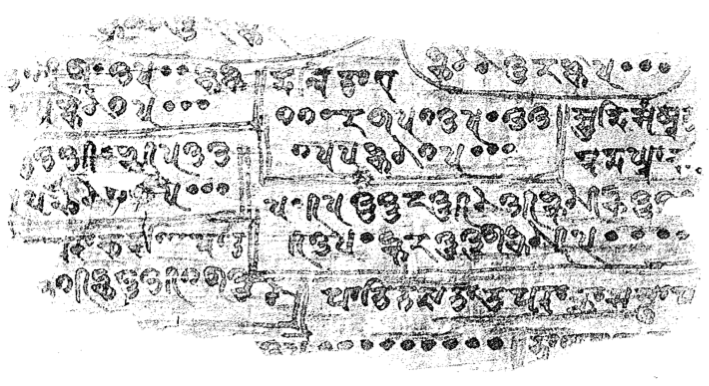
\includegraphics[scale=0.5]{bakhshali}
\end{figure}

U modernoj notaciji, algoritam kaže da za izračunati kvadratni korijen broja $q$ treba krenuti s aproksimacijom $x_0$ i zatim izračunati,
za $n\geq 0$,
\begin{align}
    a_n\: &=\: \frac{q-x^2_n}{2x_n}\\
    x_{n+1}\: &=\:x_n + a_n - \frac{a^2_n}{2(x_n + a_n)}\text.%\\
    %q\: &=\:x^2_{n+1} - \left[\frac{a^2_n}{2(x_n + a_n)}\right]^2\text.
\end{align}

Slično kao i u starobabilonskom slučaju, nema nikakvih indikacija da su staroindijski matematičari ikada iterirali gornje formule više od jedanput.
No, upravo u iteraciji leži najveća moć ove indijske metode --- algoritam kvartično konvergira\footnote{Svaka iteracija
učetverostručuje broj točnih značajnih znamenki,
pod uvjetom da nam je realna računalna aritmetika dovoljno precizna ili da radimo u racionalnoj aritmetici proizvoljne preciznosti.
Za usporedbu, poznata Newton-Raphsonova iteracijska shema konvergira kvadratno.}! Nijedan algoritam
slične efikasnosti nije bio poznat u Europi sve do 18.\ stoljeća.

\section{Moderniji pristupi}
\citat{\begin{otherlanguage}{english}
    Steve Russell certainly didn't know that his Spacewar was using a symplectic integrator.
That term wasn't invented until years later. It is serendipity that the shortest machine language program has the best numerical properties.
\end{otherlanguage}}
{Cleve Moler~\cite{spacewar}}

U ovom odjeljku ćemo razmatrati neke novije pristupe računu korijena, pri čemu mislimo uglavnom na algoritme prilagođene
izvršavanju na digitalnim računalima. Umjesto iscrpnog povijesnog pregleda svih varijanti implementiranih algoritama, usredotočit ćemo se na
nekolicinu \textsl{sui generis} algoritama i njihovih implementacija, analizirajući
njihova numerička svojstva i uspoređujući ih s onima iz odjeljka~\ref{sec:hist}. Prvo se bavimo algoritmima primarno namijenjenim računu
\emph{cjelobrojnog} korijena, a zatim algoritmom (u biti cijelom klasom algoritama) za račun realnih korijena.

\subsection{Algoritmi za cjelobrojni korijen}
\subsubsection{Algoritam s dvije varijable}
Potreba za računom kvadratnog korijena javila se vrlo rano u povijesti digitalnih računala i odgovarajuće rutine u strojnom jeziku
su ubrzo bile implementirane za računala poput EDSAC-a početkom 1950-ih godina~\cite{gower}. Takva računala tipično nisu imala ugrađen
hardver za brzu aritmetiku s pomičnim zarezom niti su podržavala instrukciju dijeljenja, pa su se tražile metode koje mogu u potpunosti
izbjeći dijeljenje i po mogućnosti koristiti samo operacije zbrajanja te bitnovnog posmaka.

Jedna takva rana metoda dolazi od ekipe predvođene Wilkesom\footnote{TODO} sa sveučilišta u Cambridgeu odgovorne za EDSAC,
inače prvo računalo s pohranjivanjem programa~\cite[str.~32]{ribaric}. Metoda je iterativna i koristi \emph{dvije} varijable te 
u potpunosti zadovoljava spomenute specifikacije. To uspijeva zahvaljujući nekim osnovnim rezultatima koje ćemo sada izvesti za
malo općenitiji slučaj izračunavanja $y/x^{1/n},\,n\in\mathbb{N}$, gdje pretpostavljamo da nas zanimaju samo pozitivni cjelobrojni rezultati, pa
je riječ o funkciji s domenom u $\mathbb{N}^2$ i kodomenom u $\mathbb N$\footnote{Ovo se može interpretirati kao račun u aritmetici
s \emph{fiksnim} zarezom, uz odgovarajuća skaliranja na početku i kraju, što je bilo uobičajeno za rana računala. Pritom želimo da algoritam
računa rezultat do na točnost $2^{-(w-1)}$, gdje je $w$ duljina riječi u bitovima, jer tako osiguravamo točan rezultat u smislu aritmetike
s fiksnim zarezom.}.

Promotrimo dvostruko iterativni proces u varijablama $a_k$ i $c_k$:
\begin{align}
        a_{k+1} &= a_k(1 + \alpha c_k)\label{eq:iter1}\\
        (y^n / x)(1 + c_{k+1}) &= a^n_{k+1}\label{eq:iter2}\text.
\end{align}
Ako $c_k\to 0$ za $k\to\infty$, onda očito vrijedi $a_k\to y/x^{1/n}$ te iz~\eqref{eq:iter1} i~\eqref{eq:iter2} lako izvodimo
\begin{equation}
    c_{k+1} = (1+c_k)(1+\alpha c_k)^n - 1\text.
\end{equation}
Bitno je da osiguramo konvergenciju; može se pokazati da ako $y^2<x<1$ (skalirano), za $|c_k|<1$ negativan imamo
\begin{equation}\label{eq:edsacscale}
    -1\leq c_{k+1}\leq(1+c_k)e^{-c_k}-1<0\text.
\end{equation}
Odabirom $\alpha=-1/n$ dobivamo kvadratnu konvergenciju ovog sustava~\cite{gower}.

Uvrštavanjem u~\eqref{eq:iter1} i~\eqref{eq:iter2}, dobivamo:
\begin{align}
    a_{k+1} &= a_k(1-c_k/n)\\
    c_{k+1} &= (1+c_k)(1-c_k/n)^n - 1\text.
\end{align}
Sada općenito vidimo da iz~\eqref{eq:edsacscale} slijedi
da su sve vrijednosti niza $c_k$ negativne te da taj niz konvergira ka $0$. Iz~\eqref{eq:iter2} pak dobivamo
$|a_k|^n<|y^n/x|$, iz čega možemo zaključiti da je $|a_k|<1$ (skalirano) čim je konačan rezultat isto takav.

Za dobiti formule specifično za račun kvadratnog korijena od $x$, odabiremo $a_0=y=x$ i $c_0=x-1$ te $n=2$, što nam daje:
% \begin{equation}
%     \begin{aligned}\label{eq:sqrtedsac}
%         a_{k+1} &= a_k\left(1-\frac12 c_k\right)\\
%         c_{k+1} &= \frac14 c^2_k(c_k-3)\text.
%     \end{aligned}
% \end{equation}
\begin{equation}
\left.
    \begin{array}{cc}
    \label{eq:sqrtedsac}
        a_{k+1} &= a_k\left(1-\frac12 c_k\right)\\
        c_{k+1} &= \frac14 c^2_k(c_k-3)\text.
\end{array}\right\}
\end{equation}
U ovom posebnom slučaju se konvergencija $a_k\to\sqrt x$ može lako provjeriti direktno po definiciji konvergencije
niza koji je monotono padajući (unutar legalnog raspona $x$-a vrijedi da su sve $c_k$ vrijednosti negativne te rastu tj.
apsolutna vrijednost niza pada) koristeći gornje rezultate o omeđenosti međurezultata; no, uočimo da to možemo pokazati
samo za $0\leq x<3$ po gornjem odabiru početnih uvjeta --- to je jedini raspon unutar kojeg je ova metoda primjenjiva (što se tiče korijena).

Ne samo da ova metoda ima relativno malu stvarnu domenu primjene, ona se također radi preciznosti često mora ograničiti još i više.
Vidimo da je iteriranje sustava~\eqref{eq:sqrtedsac} moguće korištenjem množenja, dijeljenja s potencijama od $2$ te zbrajanja i oduzimanja, što
je lako za implementirati na svim procesorima. Ipak, ova metoda, zbog korištenja dvije iteracijske varijable, može akumulirati greške za razliku
od starobabilonske metode. Konvergencija za račun korijena ovom metodom se usporava što je $x$ manji, što znači da bi trebali pred-skalirati argument
što je više moguće (do gornje granice duljine riječi), obaviti račun i na kraju skalirati natrag; štoviše, nužno je
skalirati argument tako da vrijedi $0<x<1$ (skalirano) radi osiguravanja da će konačan rezultat biti $<1$ (skalirano), čime dobivamo
traženu garanciju strojne (u smislu fiksnog zareza) preciznosti. 
Faktor skaliranja bi trebao biti parna potencija od $2$,
kako bi račun korijena bez gubitka prepolovio eksponent.

Iz svega navedenog možemo uočiti da je područje konvergencije ovog algoritma, pogotovo za nama najzanimljiviji slučaj $n=2$, izrazito usko
(u tom slučaju vidimo da je riječ o podskupu od $\{x\mid x\in\left[0,3\right>\}$ za kojeg jedino i možemo primijeniti ovaj algoritam), pa je
zaista bitno primijeniti dosta pred- i post-procesiranja kako bi se izvuklo maksimalno preciznosti iz ovog algoritma.
Gower u~\cite{gower} preporučuje ciljni raspon $(\frac12)^n\leq x<1$.
Za računala za koja je
ovaj algoritam bio
namijenjen, to je bila i jedina moguća relativno efikasna opcija.

\subsubsection{Algoritam bit-po-bit}
Sada ćemo proučiti jednu široko poznatu i implementiranu metodu za račun kvadratnog korijena, najčešće opet domene i kodomene u
$\mathbb{N}$, iako se često koristi s odgovarajućim skaliranjem i za "realne" brojeve
 na platformama gdje je moguća jedino aritmetika s fiksnim zarezom; mi ćemo podrazumijevati da radimo samo nad $\mathbb N$, pa ustvari
 dajemo algoritam za račun $\lfloor\sqrt x\rfloor$.

Riječ je o metodi kojom ljudi mogu dosta efikasno na papiru izračunati korijen, iako je sporija od svih prije obrađenih zbog toga
što u svakoj iteraciji daje samo jednu novu znamenku rezultata. Ipak, popularna je i dandanas upravo zbog svoje jednostavnosti te je
poznato da su neki rani ručni kalkulatori, poput Napierovih kosti (17.\ st.), koristili ovu metodu.
 Opisat ćemo je primjerom
u dekadskom brojevnom sustavu, a nakon toga formalizirati točan postupak za nama posebno zanimljiv binarni sustav.

\primjer{Izračunati $\sqrt{819}$.}
{Kako smo u dekadskom sustavu, znamo da troznamenkasti brojevi mogu imati najviše dvoznamekasti korijen; općenito, $k$-znamenkasti broj
može imati najviše $\lceil\frac{k}{2}\rceil$-znamenkasti korijen. Mi u biti želimo "riješiti jednadžbu" $(10x+y)^2+z=819$ za $x$ i $y$, gdje je 
"ostatak" $z$ potreban jer očekujemo da nam argument neće biti savršeni kvadrat. U tu svrhu krećemo od najznačajnije znamenke rješenja
$x$ --- koja je najveća znamenka koja, kvadrirana i pomnožena sa $100$, daje broj manji ili jednak $891$? Nalazimo da je to $x=2$, pa
uvrstimo to u jednadžbu i tražimo dalje $y$. Budući smo razriješili najznačajniji dio rezultata, možemo oduzeti dobiveni $400$ od $819$,
dobiti $40y+y^2+z=419$
i nastaviti pretragu kao prije. Tako nalazimo $y=8$ i, kako uvrštavanje u jednadžbu ne daje točno $419$,
znamo da imamo "ostatak" $z>0$. No, nama on nije bitan budući da ustvari računamo $\lfloor\sqrt{819}\rfloor$, pa je
 dovoljno vratiti naš dobiveni rezultat kao konačno rješenje.}

%\subsubsection{Općenit pseudokod}
Općenito, ovaj algoritam se svodi na iterativno traženje najvećeg jednozamenkastog
broja koji zadovoljava da mu je izračunata vrijednost preostalog dijela multinomne jednadžbe manja ili jednaka (preostalom) argumentu, sve
dok ne odredimo vrijednosti svih nepoznanica.

Možemo pokušati formalizirati ovaj pristup za slučaj baze $2$, koja nam je jedina zanimljiva radi implementacije na računalu, na temelju
jednostavne opservacije da je korijen broja $N$ ili jednak korijenu $N-1$ ili za jedan manji od njega. Obična indukcija po $N$ nam dokazuje
ovaj rezultat, no očito je riječ o presporom načinu računanja korijena, budući bi bilo potrebno napraviti onoliko \emph{rekurzivnih}
poziva koliki je $N$, sve do dolaska do baznog slučaja za $1$, uz još dodatnu provjeru kvadriranjem na kraju koja osigurava da ne vratimo
\textsl{off-by-one} rezultat! Jasno, ovakvo nešto ne dolazi u obzir, ali sada barem imamo neku ideju na čemu temeljiti dokaz, samo nam treba
"brža" indukcija.

Tvrdimo da je moguće doći do istog rezultata koristeći, umjesto opetovanog dekrementiranja argumenta u koraku, njegovo dijeljenje s $4$
tj.\ bitovni posmak za $2$ udesno, što dovodi do vremenske složenosti $O(\lg\lg N)$\footnote{$\log_2 x=\lg x$} u usporedbi s prethodnom $O(\lg N)$. Osnovna ideja je
da mi na temelju izračunatog korijena od $\lfloor\frac{N}{4}\rfloor$ možemo dobiti korijen od $N$, što opravdava korištenje potpune
indukcije na $N$ u svrhu dokaza ovog korisnijeg rezultata. Za provesti tu indukciju, moramo prvo navesti neke elementarne rezultate
na koje ćemo se pozvati (u donjim iskazima pretpostavljamo da $\mathbb{N}$ uključuje $0$).

\begin{lema}
    Za sve $a,n\in\mathbb{N}$ vrijedi:
    \begin{equation}\label{lm:1}
        a=\left\lfloor\frac{a}{n}\right\rfloor\cdot n + a \bmod n\text.
    \end{equation}
\end{lema}

\begin{lema}
    Za sve $a,n\in\mathbb{N}$ vrijedi:
    \begin{equation}\label{lm:2}
        0 \leq a \bmod n \land a \bmod n < n\text.
    \end{equation}
\end{lema}

\begin{teorem}\label{tm:isqrt1}
    Korijen od $x\in\mathbb N$ je ili $2r$ ili $2r+1$, gdje $r^2\leq\left\lfloor\frac{x}{4}\right\rfloor < (r+1)^2$. Preciznije,
    ako je $x < (2r+1)^2$, tada je korijen $2r$, a inače je korijen $2r+1$~\cite{sqrtproof}.
\end{teorem}
\begin{proof}
    Potpunom indukcijom po $x$. U baznom slučaju, za $x=0$, imamo da je korijen dakako $0$.

    Pretpostavka indukcije nam je da kada tvrdnja vrijedi za sve brojeve manje od $x$, tada ona vrijedi i za $x$.
    Obzirom da imamo dva različita slučaja u tvrdnji, korak provodimo po slučajevima.
    \paragraph{Slučaj 1: $x<(2r+1)^2$}
    
    U ovom slučaju tvrdimo da je korijen $2r$, pa valja pokazati da vrijedi $(2r)^2\leq x < (2r+1)^2$. Desnu nejednakost već pretpostavljamo,
    a prva slijedi osnovnim algebarskim manipulacijama:
    \begin{align*}
        r^2 &\leq \left\lfloor\frac{x}{4}\right\rfloor &\\
        r^2\cdot 4 &\leq \left\lfloor\frac{x}{4}\cdot 4\right\rfloor &\\
        (2r)^2 &\leq \left\lfloor\frac{x}{4}\right\rfloor\cdot 4 &\\
        (2r)^2 &\leq (x - x \bmod 4) & \text{po \eqref{lm:1}}\\
        x - x \bmod 4 &\leq x & \text{po \eqref{lm:2}}\\
        (2r)^2 &\leq  x\text.&
    \end{align*}

    \paragraph{Slučaj 2: $x \geq (2r+1)^2$}

    Sada tvrdimo da je korijem $2r+1$, pa dokazujemo da vrijedi $(2r+1)^2 \leq x < (2r+2)^2$. Prva nejednakost je sada trivijalno zadovoljena,
    a za drugu možemo postupiti ovako:
    \begin{align*}
        \left\lfloor\frac{x}{4}\right\rfloor &< (r+1)^2 & \text{po pretpostavci indukcije}\\
        \left\lfloor\frac{x}{4}\right\rfloor + 1 &\leq (r+1)^2 \bigg/\cdot 4 &\\
        \left\lfloor\frac{x}{4}\right\rfloor\cdot 4 + 4 &\leq (r+1)^2\cdot 4 = (2r+2)^2 &\\
        x - x \bmod 4 + 4 &\leq (2r+2)^2 & \text{po \eqref{lm:1}}\\
        x &\leq (2r+2)^2 + x \bmod 4 - 4 &\\
        (2r+2)^2 + x \bmod 4 - 4 &< (2r+2)^2 & \text{po \eqref{lm:2}}\\
        x &< (2r+2)^2\text.&
    \end{align*}
\end{proof}

Sada imamo zgodan algoritam za računati korijene koji je direktno primjenjiv i za ručno računanje, iako najvjerojatnije zahtijeva papir
za pamćenje rezultata za veće argumente. Vidimo da algoritam napreduje dijeljenjem preostalog dijela argumenta (u potproblemu) s $4$, što
odgovara bitovnom posmaku za 2 udesno i stoga se lako vizualizira i izvodi u računalu, iako za ljude možda nije najprirordnije raditi u bazi $2$.
U tom slučaju računamo u bazi $10$ i, umjesto $4$, za djelitelja odabiremo $100$ kao prvi savršeni kvadrat te baze i svi ostali rezultati slijede
na analogan način. Pseudokod generičkog algoritma za bazu $B$ glasi:
\begin{algorithm}
    \floatname{algorithm}{Algoritam}
    \caption{Algoritam $\mathsf{isqrt}$ za cjelobrojni kvadratni korijen od $N$ u bazi $B$}\label{alg:isqrt1}
    \begin{algorithmic}
    \Require $N \geq 0$
    \If{$N = 0$}
        \State $rezultat \gets 0$
    \Else
        \State $z \gets \left\lfloor\dfrac{N}{B^2}\right\rfloor$
        \State $r_2 \gets B \cdot \mathsf{isqrt}(z)$
        \State $r_3 \gets r_2 + 1$
        \If{$N < r_3^2$}
            \State $rezultat \gets r_2$
        \Else
            \State $rezultat \gets r_3$
        \EndIf
    \EndIf
    \end{algorithmic}
\end{algorithm}

Jasno, ovo je čisto rekurzivna implementacija teorema~\ref{tm:isqrt1} dokazanog indukcijom za koju ne očekujemo jako dobre performanse upravo zbog
uporabe rekurzije. Usredotočimo se na slučaj za $B=2$ i prevedimo algoritam~\ref{alg:isqrt1} u iterativni pseudokod uz nekoliko optimizacija: rezultat
je algoritam~\ref{alg:isqrt2}.
\begin{algorithm}
    \floatname{algorithm}{Algoritam}
    \caption{Algoritam $\mathsf{isqrt}$ za $B=2$, iterativna varijanta za $32$-bitnu arhitekturu~\cite{guysqrt}}\label{alg:isqrt2}
    \begin{algorithmic}[1]
    \Require $N \geq 0$
    \State $op \gets N$
    \State $rezultat \gets 0$
    \State $jedinica \gets 2^{30}$
    \While{$jedinica > op$}
        \State $jedinica \gets \left\lfloor\frac{jedinica}{4}\right\rfloor$
    \EndWhile

    \While{$jedinica\neq 0$}
        \If{$op \geq rezultat + jedinica$}
            \State $op \gets op - (rezultat + jedinica)$
            \State $rezultat \gets rezultat + 2 \cdot jedinica$\label{line:rezupd}
        \EndIf
        \State $rezultat \gets \left\lfloor\frac{rezultat}{2}\right\rfloor$
        \State $jedinica \gets \left\lfloor\frac{jedinica}{4}\right\rfloor$
    \EndWhile
    \end{algorithmic}
\end{algorithm}

Objasnimo pobliže što se dogodilo u transformaciji iz algoritma~\ref{alg:isqrt1} u algoritam~\ref{alg:isqrt2}. Prva očita stvar je da, umjesto kretanja
od točno najvišeg ne-nula bita od $N$\footnote{U praksi se ovaj algoritam izvodi na računalima gdje ćemo, zbog fiksnih
i relativno malih širina registara, uvijek kretati od najviše bitovne pozicije (ovo ima smisla do oko $32$ bita).
Naravno da onda postoje i varijante u kojima se pokušava na razne načine
zaobići potreba prolaska od najvišeg bita uz obavljanje cijelog računa svaki put, što može dovesti do ubrzanja, ali samo uz povećanje
memorijskih zahtjeva jer nam tada treba barem nekakva konstantna tablica vrijednosti u memoriji.
Jedan takav algoritam, zasnovan na tablici i malom broju računskih operacija,
bit će obrađen zadnji.}, što bi zahtijevalo i inicijalno izračunavanje indeksa te pozicije, mi jednostavno možemo krenuti od najvišeg bita registra.
Preciznije, budući da znamo da ćemo u koraku dijeliti s $4$ tj.\ posmaknuti sve bitove za $2$ mjesta udesno (u niskorazinskim implementacijama), dovoljno
je započeti na najznačajnijoj grupi od dva bita, s tim da mi pamtimo \emph{niži} indeks i postavljamo jedinicu tamo.  To nam omogućuje laganu provjeru
kraja algoritma: kada je ostatak bitova iz $jedinica$ kompletno u $0$, više nema potrebe ništa računati i prekidamo algoritam.

Dualno, ne zanimaju nas ni najviši $0$-bitovi iz $N$ jer oni ne mogu doprinijeti korijenu, pa se pomičemo po dva bita udesno dok ne "udarimo" u neki 
par ne-nula bitova iz $N$, pri čemu je $n$ indeks najviše bit-pozicije u $N$. U tom trenutku dakle, nakon završetka prve \textbf{while} petlje,
znamo par indeksa među kojima je indeks pozicije najvišeg bita u $N$. Sada idemo, unutar iduće petlje, obaviti sve korake dok ne iscrpimo
sve relevantne parove bitova. Treba objasniti točno što druga petlja radi, jer nije inicijalno očito da ima ikakve veze s algoritmom~\ref{alg:isqrt1},
iako vidimo da se korektno pomičemo po dva bita udesno. Kao prvo, stavimo $N=x^2+r$, gdje $x^2\leq N < (x+1)^2$ i $r$ je "ostatak".
Mi dakle tražimo bitove $x=a_0,\dotsc ,a_n,\,a_i\in\{2^i,0\}$. To radimo tako da održavamo aproksimaciju $x$-a $P_m=a_n+a_{n-1}+\dotsb+a_m$.
Kako napredujemo od \emph{viših} bit-pozicija prema nižim, imamo $P_m=P_{m+1}+a_m$, gdje moramo odlučiti je li $a_m=0$ ili je $a_m=2^m$.
To očito možemo na temelju nejednakosti $(P_{m+1}+2^m)^2 \leq N$ --- ako je ona istinita, $a_m=2^m$, a inače $a_m=0$. Ovo bi bilo dovoljno za
osnovni iterativni algoritam, ali tada bismo morali u svakom koraku kvadrirati dosadašnju aproksimaciju, što nije nužno ako iskoristimo činjenicu
da su znamenke u bazi $2$ invarijantne na kvadriranje i da kvadrat aproksimacije možemo lako ažurirati. Uočimo da vrijedi
\begin{equation}\label{eq:optim1}
    \begin{aligned}
    (P_m+a_{m-1})^2 &\leq N\\
    \iff 2P_ma_{m-1}+a^2_{m-1} &\leq N-P^2_{m-1}-2P_{m+1}a_m-a^2_m\text.
    \end{aligned}
\end{equation}
Dakle, ako želimo brzo otkriti treba li odabrati $2^{m-1}$ ili $0$, treba nam razlika $\Delta_{m-1}$ između desne strane jednadžbe \eqref{eq:optim1}
za dvije uzastopne aproksimacije. Nalazimo
\begin{equation}\label{eq:optim2}
    \begin{aligned}
    \Delta_{m-1}&=N-P^2_{m+1}-a^2_m-2P_{m+1}a_m-\left(N-P^2_{m+2}-a^2_{m+1}-2P_{m+2}a_{m+1}\right)\\
    &=P^2_{m+2}-P^2_{m+1}-a^2_m+a^2_{m+1}+2a_{m+1}P_{m+2}-2a_mP_{m+1}\\
    &=-(2a_mP_{m+1}+a^2_m)\text.
    \end{aligned}
\end{equation}
To znači da u svakoj iteraciji oduzimamo izraz~\eqref{eq:optim2} od varijable $op$ inicijalizirane sa $N$ (uočimo da je izraz $0$ kada $a_m=0$, pa ustvari
ne radimo ništa u tom slučaju). No sada želimo što brže izračunati taj izraz, po mogućnosti bez potrebe ikakvog množenja (i kvadriranja), što je moguće
inkrementalnim računanjem dviju pomoćnih varijabli, od kojih svaka odgovara jednom pribrojniku u~\eqref{eq:optim2}. Konkretno,
\begin{equation}\label{eq:optim3}
    \begin{aligned}
    rezultat_m &= 2a_mP_{m+1}=P_{m+1}2^{m+1}=P_{m+1}2^{m+1}=(P_{m+2}+a_{m+1})2^{m+1}\\
    &=P_{m+1}\cdot 2^{m+1}+a_{m+1}2^{m+1}\\
    &=\begin{cases}
        \frac{rezultat_{m+2}}{2},&\text{ako $a_{m+1}=0$}\\
        \frac{rezultat_{m+2}}{2} + a_{m+1}2^{m+1},&\text{inače}\text.
    \end{cases}
    \end{aligned}
\end{equation}
Evidentno je da nam druga varijabla $jedinica$ treba odgovarati izrazu $a_{m+1}2^{m+1}$ koji je jednak $2^{m+1}\cdot 2^{m+1}=4^{m+1}$ jer
u ovom trenutku ažuriranja znamo da smo odabrali $a_{m+1}=2^{m+1}$ (inače ne bi bilo nikakvog ažuriranja). Stoga na kraju petlje još moramo imati
\begin{equation}
    jedinica_m=4^m=\frac{jedinica_{m+1}}{4}\text.
\end{equation}
Sada vidimo da u~\eqref{eq:optim3} možemo optimalno ažurirati $rezultat$ bez potrebe za množenjem:
\begin{equation}
    \begin{cases}
        rezultat_{m+2}/2,&\text{ako $a_{m+1}=0$}\\
        rezultat_{m+2}/2 + jedinica_{m+1},&\text{inače}\text.
    \end{cases}
\end{equation}
Očito, sada je moguće izračunati $\Delta$ vrijednost ažuriranja kao $jedinica+rezultat$ u svakoj iteraciji te će na kraju $rezultat$ ujedno i
predstavljati konačnu (najbolju cjelobrojnu) aproksimaciju korijena $x$. Napomenimo da bi sve operacije koje uključuju množenje ili dijeljenje s
potencijom od $2$ trebale biti zamijenjene odgovarajućim bitovnim posmakom u stvarnim implementacijama.

Iako se čini da ovaj algoritam ne napreduje suviše brzo (ne pogađa inicijalnu aproksimaciju koju zatim profinjuje), njegova je
glavna prednost to što ima fiksan broj iteracija petlje
(ovisan samo o duljini registara ciljne arhitekture) i stoga relativno lako odredivo ukupno
vrijeme izvršavanja na jednostavnijim, danas uglavnom ugradbenim arhitekturama. Idući algoritam može postići bolje performanse na većini
modernih strojeva koristeći "informiraniju" progresivnu aproksimaciju.

%\subsection{CPython-ov algoritam}
\subsubsection{Algoritmi s adaptivnom preciznosti}
\citat{\begin{otherlanguage}{english}
    The integer square root is a common number-theoretic primitive, useful for example in primality testing.
This is something I've had to code up myself multiple times, and is also something that's quite easy to get wrong,
or implement in a way that's inefficient for large inputs~\cite{mdickisqrt}.
\end{otherlanguage}}{Mark Dickinson}

Trenutna verzija CPythona --- referentne implementacije virtualnog stroja za programski jezik Python --- koristi zanimljivu varijantu 
algoritma~\ref{alg:isqrt2} za račun cjelobrojnog kvadratnog korijena~\cite{Cpythonisqrt}. Naime, radi se o \emph{adaptivnom} algoritmu
koji umjesto posmaka za fiksni broj mjesta koristi varijabilni posmak $s$ koji se smanjuje kako algoritam napreduje. Iteracije se baziraju
na Newtonovoj-Raphsonovoj metodi i koristi se puno brža metoda u posebnom slučaju kada je argument manji od $2^{64}$; naime, Python interno podržava
cjelobrojnu aritmetiku proizvoljne preciznosti, no raditi račun u proizvoljno visokoj preciznosti kada bi se mogao izvesti i u puno manjoj
(idealno strojnoj) je rastrošno, pa algoritam ustvari adaptivno povećava preciznost računa. Također postoji posebna, vrlo kratka
i efikasna varijanta koja se sastoji samo od najosnovnijih aritmetičkih operacija i ne sadrži grananja.
U samom Pythonu, ova funkcija je dostupna kao \texttt{math.isqrt} od verzije 3.8.

CPython-ov algoritam se temelji na sličnoj ideji kao prethodni bit-po-bit algoritam, samo što sada ne želimo koristiti fiksni djelitelj
za dobivanje manjeg korijena iz kojeg se onda izvlači željeni korijen, već želimo u svakoj iteraciji izračunati aproksimaciju od
$\lfloor N/4^f\rfloor$ za neki pozitivni $f$ koji opada kako iteracije napreduju te je na kraju $0$. Također, dopuštamo da se konačan
rezultat računa progresivnim aproksimacijama u svakoj iteraciji, gdje je akumulacija greške kontrolirana i dokazivo omogućuje izbavljanje
točnog rezultata na samom kraju. Ovaj algoritam 
koristi te ideje kombinirane s osnovnom Heronovom metodom da izračuna tzv.\ skoro-korijen od $N$, po definiciji iz~\cite{mdickpaper}:
\begin{definicija}
    Neka je $N\in\mathbb N$. Kažemo da je $a\in\mathbb N$ \emph{skoro-korijen} od $N$ ako vrijedi 
    \begin{equation*}
        (a-1)^2 < N < (a+1)^2\text.
    \end{equation*}
\end{definicija}
Očito nije problem dobiti cjelobrojni korijen iz skoro-korijena. Idući teorem govori, slično kao~\autoref{tm:isqrt1} za neadaptivni slučaj,
kako dobiti skoro-korijen iz skoro-korijena određenog kvocijenta.
\begin{teorem}
    Neka su $N,k\in\mathbb N$ i $4k^4 \leq N$. Neka je $b$ skoro-korijen od $\lfloor N/4k^4\rfloor$. Tada je 
    \begin{equation}
        a=kb+\left\lfloor\frac{N}{4kb}\right\rfloor
    \end{equation}
    skoro-korijen od $N$.
\end{teorem}
\begin{proof}
    Po definiciji skoro-korijena imamo
    \begin{equation}
        (b-1)^2 < \left\lfloor\frac{N}{4k^2}\right\rfloor < (b+1)^2\text.
    \end{equation}
    Kako je $(b+1)^2$ cijeli broj, vrijedi
    \begin{equation}\label{eq:py1}
        (b-1)^2 < \frac{N}{4k^2} < (b+1)^2\text.
    \end{equation}
    Množenjem~\eqref{eq:py1} sa $4k^2$ i uzimanjem korijena dobivamo
    \begin{equation}
        2k(b-1) < \sqrt{N} < 2k(b+1)
    \end{equation}
    iz čega slijedi
    \begin{equation}\label{eq:py2}
        |2kb - \sqrt{N}| < 2k\text.
    \end{equation}
    Kvadriranjem i dijeljenjem~\eqref{eq:py2} s $4kb$ dobivamo
    \begin{equation}\label{eq:py3}
        0 \leq kb + \frac{N}{4kb} - \sqrt{N} < k/b,
    \end{equation}
    što povlači
    \begin{equation}
        -1 < kb + \left\lfloor\frac{N}{4kb}\right\rfloor - \sqrt{N} < k/b\text.
    \end{equation}
    Po definiciji od $a$ iz~\eqref{eq:py3} dobivamo 
    \begin{equation}\label{eq:py4}
        -1 < a - \sqrt{N} < k/b\text.
    \end{equation}
    
    Još nam treba činjenica da $k/b\leq1$. Nju možemo dobiti kombiniranjem pretpostavke da je $4k^4 \leq N$ i desne strane iz~\eqref{eq:py1},
    čime dobivamo $k^2 < (b+1)^2\implies k < b+1\implies k\leq b\implies k/b\leq 1$. Konačno, iz~\eqref{eq:py4} sada slijedi
    \begin{equation}
        -1 < a - \sqrt{N} < 1\text.
    \end{equation}
\end{proof}

Slijedi pseudokod rekurzivne verzije algoritma kojeg CPython koristi, iako je u implementaciji korištena \emph{iterativna} varijanta koju nećemo
dalje analizirati.
\begin{algorithm}
    \floatname{algorithm}{Algoritam}
    \caption{$\mathsf{nsqrt}$ algoritam za račun skoro-korijena (rekurzivna verzija)~\cite{mdickpaper}}\label{alg:nsqrt}
    \begin{algorithmic}[1]
    \Require $N \geq 0$
    \If{$N < 4$}
        \State $rezultat \gets 1$
    \Else
        \State $e \gets \lfloor(N.bitova - 3) / 4\rfloor$
        \State $b \gets nsqrt(\lfloor N / 2^{2e+2}\rfloor)$
        \State $rezultat \gets (b \cdot 2^e) + \left\lfloor \dfrac{\lfloor N / 2^{e+2}\rfloor}{b}\right\rfloor$
    \EndIf
    \end{algorithmic}
\end{algorithm}
Kada dobijemo skoro-korijen ovim algoritmom, a želimo cjelobrojni korijen, samo provjerimo je li kvadrat rezultata veći od argumenta ili ne;
ako je, moramo ga umanjiti za $1$ za dobiti cjelobrojni korijen.
U algoritmu~\ref{alg:nsqrt} je odabran $k=2^e$ za $e=\lfloor(N.bitova - 3) / 4\rfloor$ kako bi se sva množenja i dijeljenja mogla svesti
na bitovne posmake i kako bi broj iteracija bio što manji. Drugim riječima, pronađen je najveći $k$ koji je potencija od $2$ i koji
zadovoljava $4k^4 \leq n$. $rezultat$ se dobiva sumiranjem $kb$ sa $\left\lfloor\dfrac{N}{4kb}\right\rfloor$, što sada odgovara rezultatu
$\mathsf{nsqrt}$ poziva $b$ posmaknutim ulijevo za $e$ mjesta, jer je $k=2^e$, odnosno $n$ posmaknutom udesno za $e+2$, što odgovara
dijeljenju s $4k$, nakon čega dolazi dijeljenje s  $b$.

CPython također sadrži posebne slučajeve ovog algoritma za "manje" argumente tj.\ najčešće korištene brojeve koji su direktno hardverski
podržani (bez potrebe korištenja aritmetike proizvoljne preciznosti). U tim slučajevima možemo jednostavno "razmotati" algoritam~\ref{alg:nsqrt} fiksni
broj puta (za kojeg se zna da se uvijek dobiva točan rezultat za npr.\ $32$ ili $64$ bita) i zapisati ga kao konstantan niz naredbi. Vidimo da je to onda,
barem što se tiče prosječnog slučaja i apsolutne prostorne složenosti, najefikasniji algoritam za cjelobrojni korijen kada radimo s hardverskim
cijelim brojevima\footnote{Postoji još efikasnija varijacija u terminima ukupnog \emph{broja} (ne i pojedine složenosti!) instrukcija, koja korištenjem jednog
množenja i jednog
dijeljenja uz pomoćnu tablicu može postići impresivne performanse na nekim arhitekturama; k\^od je u~\cite{mdickpaper}.}.

\subsection{Algoritmi za realan korijen}
Zadnja klasa algoritama kojih ćemo proučiti je šire primjene od većine prošlih --- namijenjena je uporabi na modernim računalima s dostupnom (i brzom)
jedinicom za račun s pomičnim zarezom --- te je stoga prilagođen za davanje aproksimacija realnog korijena. Najčešće nas zanimaju samo
približne vrijednosti u takvim primjenama, a općenito nije ni teoretski moguće dati točne rezultate, za razliku od cjelobrojnog korijena. 

Kako je uobičajeno da procesori implementiraju podršku za aritmetiku s pomičnim zarezom na temelju
IEEE 754 standarda, želimo iskoristiti što više specifičnosti te reprezentacije za dobiti što bolju preciznost (slično kao što smo ovisili o binarnom
prikazu cijelih brojeva radi obavljanja brzih bitovnih posmaka i povećanja preciznosti u prošlim algoritmima). Napomenimo također da želimo izbjeći
bilo kakve skupe operacije s pomičnim zarezom, a to su množenje i pogotovo dijeljenje! Uzimamo u obzir račun u jednostrukoj preciznosti, dakle s
\texttt{float} tipom u C-u, iako se sve ideje ispod mogu implementirati za proizvoljan binaran format po IEEE 754 standardu.
\subsubsection{Direktna aproksimacija }
S tim na umu, prvo razmatramo algoritam koji lukavo koristi IEEE 754 reprezentaciju kako bi nakon nekolicine brzih operacija dao iznenađujuće
dobru aproksimaciju korijena, i to bez korištenja ikakve iterativne metode!
\begin{algorithm}
    \floatname{algorithm}{Algoritam}
    \caption{$\mathsf{sqrt}$ algoritam za račun aproksimacije realnog korijena~\cite{lomont}}\label{alg:sqrt}
    \begin{algorithmic}[1]
    \Require $x \geq 0$
    \State $repr \gets \text{bitovi iz binarne IEEE 754 reprezentacije broja $x$}$
    \State $repr \gets repr - repr \cdot 2^{23}$
    \State $repr \gets \lfloor\frac{repr}{2}\rfloor$
    \State $repr \gets repr + repr \cdot 2^{29}$
    \State $rezultat \gets \text{broj u IEEE 754 formatu konstruiran iz binarne reprezentacije $repr$}$
    \end{algorithmic}
\end{algorithm}
Algoritam~\ref{alg:sqrt} se čini poprilično kriptičnim i najvjerojatnije nije odmah jasno kako bi mogao rezultirati nečim blizu korijena od $x$, pa
ponovimo par osnovnih stvari o IEEE 754 formatu. Po specifikaciji, \texttt{float} je definiran kao $32$-bitni niz u kojem je najviši bit predznaka $P$,
zatim slijedi $8$ bitova eksponenta $E$ s otklonom od $127$ te konačno $23$ najniža bita \emph{mantise} $M$. Sveukupno dakle, imamo 
%TODO: treba tikz skica formata ovdje, sa slovnim oznakama dijelova u ćelijama
\begin{equation}
    x = (2^{23} + M)2^{E-127},
\end{equation}
pri čemu treba imati na umu da je nama $P=0$ zbog nužne nenegativnosti $x$-a te da
 cijeli signifikand broja $x$ ustvari ima $24$ bita, pri čemu je najznačajniji implicitno $1$, pa se pamte
samo niža $23$ bita u mantisi $M$. Kako je $\sqrt{x} = \sqrt{2^{23}+M}\cdot 2^{\frac{E-127}{2}}$, želimo nekako što brže 
od $x$ doći do rastava na dio bitova koji se tiče samo eksponenta i dio koji se tiče mantise. U tu svrhu možemo jednostavno
podijeliti našu bitovnu reprezentaciju s $2^{23}$, čime smo ustvari doveli \emph{otklonjeni} eksponent do najniže bit-pozicije i sada
lako njime manipuliramo tj.\ normaliziramo oduzimanjem $127$. Jedino što preostaje napraviti je podijeliti s $2$ (prepolavljamo eksponent),
dodati natrag $127$ i pomnožiti sa $2^{23}$ kako bi se eksponent vratio na svoje pravo mjesto u bitovnoj reprezentaciji. Ovaj postupak
dakako općenito neće korektno izračunati korijen mantise, ali imamo i veći problem: inicijalnim dijeljenjem s $2^{23}$ mi gubimo \emph{sve} informacije
o mantisi! Srećom, uz malo algebre, lako vidimo da je opisani račun moguće izraziti na način u kojem ne izgubimo te informacije, a uz to dobijemo
i dobru aproksimaciju korijena mantise:
\begin{equation}\label{eq:sqrtshift}
    \left(\frac{\frac{x_{repr}}{2^{23}} - 127}{2} + 127\right) \cdot 2^{23} = \frac{x_{repr} - 2^{23}}{2} + 2^{22}\cdot 128\text.
\end{equation}
Sada možemo vidjeti da račun i konstante iz~\ref{alg:sqrt} odgovaraju upravo desnoj strani u~\eqref{eq:sqrtshift} (dakako, taj bi račun u 
stvarnosti trebalo implementirati isključivo bitovnim posmacima, pored jednog nužnog zbrajanja).

Metode temeljene na ovakvim trikovima daju jako dobre rezultate aproksimacije, koji postaju tim bolji što bolje odaberemo
određenu korekcijsku konstantu $k$ koju jednostavno možemo dodati bitovnoj reprezentaciji u 
algoritmu~\ref{alg:sqrt} prije pretvaranja u rezultat. Štoviše, detaljnija analiza iz~\cite{lomont} 
 pokazuje da na ovaj način ustvari postižemo po dijelovima linearnu aproksimaciju korijena, gdje se kao sljedeći korak ka poboljšanju
 preciznosti čini poprilično prirodno uzeti Newton-Raphsonovu metodu i onda je iterirati potreban broj puta. Ipak, takav pristup nije optimalan
 za \emph{direktan} račun korijena, već za račun njegove \emph{recipročne} vrijednosti.

\subsubsection{Korijen iz recipročnog korijena}
Ovdje razmatran
algoritam brzo nalazi jako dobru aproksimaciju \emph{recipročne} vrijednosti korijena, iz koje je onda trivijalno dobiti s\^am korijen:
\begin{equation}
    \sqrt{x} = \frac{1}{\sqrt{x}} \cdot x\text.
\end{equation}
Pri samom računu recipročne vrijednosti koristimo do sada viđene tehnike: Newton-Raphsonove iteracije (ekvivalentno Heronovoj metodi) i prethodne
trikove vezane za IEEE 754 format, no ovoga si puta zbog rada u realnoj domeni ne možemo priuštiti (nužno dosta velike) tablice u klasičnom smislu,
već trebamo pronaći dobru (jednu)
\emph{polaznu vrijednost} aproksimacije. Dapače, ispada da je upravo u tom odabiru moć ovog fascinantnog algoritma: uz samo \emph{jednu} iteraciju
Newton-Raphsona, postiže se relativna greška od $0.18\%$! Algoritam je implementiran u~\autoref{code:invsqrt}, a detaljna analiza preciznosti i ovisnosti
o odabranoj "magičnoj konstanti" za inicijalnu aproksimaciju se može pronaći u~\cite{lomont}.

\section{Implementacije i usporedbe}
Za kraj ovog rada, implementiramo tri glavna pristupa računu (cjelobrojnog ili realnog) korijena uz neke manje varijacije
u C++-u i uspoređujemo njihove performanse. Sav k\^od i Python skripte za mjerenje se nalaze u
\href{https://github.com/mraguzin/mathsoft-esej2}{repozitoriju} ovog rada.

\subsection{Algoritam bit-po-bit}
\begin{lstlisting}[language=C++, caption=C++ implementacija bit-po-bit algoritma]
int32_t sqrt(int32_t N)
{
	int32_t op = N;
	int32_t rezultat = 0;

	int32_t jedinica = 1 << 30;
	while (jedinica > op) jedinica >>= 2;

	while (jedinica != 0) {
		if (op >= rezultat + jedinica) {
			op -= rezultat + jedinica;
			rezultat += 2 * jedinica;
		}

		rezultat >>= 1;
		jedinica >>= 2;
	}

	return rezultat;
}
\end{lstlisting}
%Srednje vrijeme računa korijena za ovaj algoritam, kroz $16$ iteracija, je $0.016875\ \mu s$ (ono ne ovisi o veličini argumenta).

\subsection{Rekurzivni Heronov algoritam}
Ovo je rekurzivna verzija algoritma kojeg koristi CPython, samo bez adaptivnosti za proizvoljne veličine argumenta i u rekurzivnoj izvedbi.
Samim time, glavna prednost ovog pristupa nije do kraja iskorištena, a rekurzivni pozivi očito koštaju dovoljno da dovedu prosječno vrijeme izvršavanja
ovog algoritma za najveće argumente (budući da vrijeme ovdje ovisi o veličini argumenta) premašuje ono od bit-po-bit-algoritma za iste argumente.
\begin{lstlisting}[language=C++, label=code:nsqrt, caption=Rekurzivna C++20 implementacija Heronove metode]
int nsqrt(unsigned int N)
{
    if (N < 4)
        return 1;

    int bitova = sizeof(int)*8 - std::countl_zero(N);
    int e = (bitova - 3) >> 2;
    int b = nsqrt(N >> ((e << 1)+2));

    return (b << e) + (N >> (e+2)) / b;
}

int isqrt(unsigned int N)
{
    int skoro = nsqrt(N);
    return skoro*skoro <= N ? skoro : skoro - 1;
}
\end{lstlisting}
\autoref{code:nsqrt} treba kompajlirati koristeći C++20 kompajler, budući da ovisimo o brzoj funkciji za brojanje vodećih $0$-bitova, koja je pogotovo
važna u situacijama gdje bi ovaj algoritam bio primijenjen na ulazni cijeli broj proizvoljne duljine, no kako mi koristimo fiksnu (strojnu) preciznost,
dovoljno nam je koristiti standardiziranu C++ funkciju \texttt{countl\_zero} za tu svrhu, koja će se svesti na minimalan niz instrukcija.
Srednje vrijeme izvršavanja značajno varira i u nekim instancama daje bolje rezultate od bit-po-bit
algoritma; za stabilizirati ove performanse bi trebalo koristiti iterativnu verziju, što CPython i čini. Nadalje, za strojne brojeve možemo
primjeniti prije spomenuto "razmotatavanje" rekurzivnih poziva
u \autoref{code:nsqrt} i tako dobiti (za $32$-bitne brojeve) k\^od iz \autoref{code:sqrt32}.
\begin{lstlisting}[language=C++, label=code:sqrt32, caption=C++20 implementacija algoritma za $32$-bitne argumente~\cite{mdickpaper}]
uint32_t sqrt32(uint32_t N)
{
    unsigned e = std::countl_zero(N) >> 1;
    unsigned m = N << (e << 1);
    unsigned a = 1 + (m >> 30);
    a = (a << 1) + (m >> 27) / a;
    a = (a << 3) + (m >> 21) / a;
    a = (a << 7) + (m >> 9) / a;
    a >>= e;

    return a*a <= N ? a : a - 1; // odredimo cjelobrojni korijen iz skoro-korijena
}
\end{lstlisting}
Očekivano, \autoref{code:sqrt32} daje najbolje performanse u mjerenjima.


\subsection{Algoritmi za realan korijen}
Ovdje se bavimo implementacijom obrađenih varijanti algoritma za realni korijen, i to samo onih temeljenih na dobrom odabiru "magične konstante"
koja može služiti kao početna aproksimacija za Newton-Raphsonove iteracije ili jednostavno kao parametar $k$ za dodati bitovnoj reprezentaciji
broja s pomičnim zarezom na kraju algoritma~\ref{alg:sqrt}.
\begin{lstlisting}[language=C++, label=code:sqrt, caption=C++20 implementacija direktne aproksimacije realnog korijena]
float sqrt(float x)
{
    int repr = std::bit_cast<int>(x);
    repr -= 1 << 23;
    repr >>= 1;
    repr += 1 << 29;

    return std::bit_cast<float>(repr);
}
\end{lstlisting}

\begin{figure}[h]
\begin{lstlisting}[language=C++, label=code:invsqrt, caption=C++20 implementacija aproksimacije korijena preko recipročne vrijednosti]
float sqrt2(float x)
{
    float pola = 0.5f * x;
    int i = std::bit_cast<int>(x);
    i = 0x5f375a86 - (i >> 1);
    float reciproc = std::bit_cast<float>(i);
    reciproc *= 1.5f - pola*reciproc*reciproc;

    return x*reciproc;
}
\end{lstlisting}
\end{figure}

\section{Rezultati mjerenja i zaključak}
Na kraju sabiremo sva obavljenja mjerenja implementiranih algoritama u tablicu xyz
\begin{table}[t]
    %\begin{tabular}{lll}
    \begin{tabular}{|c|c|c|}
    \hline
    \multicolumn{3}{|c|}{\textbf{Rezultati mjerenja}}\\ \hline
    Algoritam & Vrijeme & Preciznost \\ \hline
    %\multicolumn{1}{|l}{Algoritam} & Vrijeme & \multicolumn{1}{l|}{Preciznost} \\ \hline
    %\multicolumn{1}{|l}{}          &         & \multicolumn{1}{l|}{}           \\ \hline
    \end{tabular}
\end{table}

\autoref{code:invsqrt} dolazi iz~\cite{walczyk2018improving}, gdje autori razmatraju kako se dolazi do "magične konstante"
\verb|0x5f375a86| i može li se izvesti neka bolja vrijednost, uz različit broj Newton-Raphson iteracija. Cilj je u tome da se postigne što
veća preciznost uz što manje iteracija te skupih operacija s pomičnim zarezom općenito; vidimo da \autoref{code:invsqrt} koristi mali
broj množenja, no taj se broj povećava kako uvodimo više iteracija te zbog toga što na kraju moramo pomnožiti s $x$ ako nas zanima korijen, a ne
(samo) recipročni korijen, pa treba pronaći dobar balans između broja operacija i tražene preciznosti.

Na kraju valja napomenuti da danas praktički sve arhitekture generalnih procesora imaju ugrađenu instrukciju za vađenje kvadratnog korijena, kao
i njegove recipročne vrijednosti, koja daje preciznije rezultate i brža je od svih navedenih algoritama za rad s pomičnim zarezom. Ipak, ovakvi
algoritmi su nužni na mnogim ugradbenim i jednostavnijim sustavima (FPGA i sl.) koji nemaju takve sposobnosti.



\printbibliography

\end{document}